% Presentatie Project 7 (tussentijds)
\documentclass{beamer}

\mode<presentation>

\usepackage[dutch]{babel}
%\usepackage{beamerthemesplit}
\usetheme{Berlin}
\useinnertheme{rounded}
\usecolortheme{rose}

\setbeamertemplate{footline}%[frame number]
{
  \hbox{%
  \begin{beamercolorbox}[wd=.5\paperwidth,ht=2.25ex,dp=1ex,center]{title in head/foot}%
    \usebeamerfont{title in head/foot}\insertshorttitle
  \end{beamercolorbox}%
  \begin{beamercolorbox}[wd=.5\paperwidth,ht=2.25ex,dp=1ex,right]{date in head/foot}%
    \usebeamerfont{date in head/foot}
    \insertframenumber{} / \inserttotalframenumber\hspace*{2ex} 
  \end{beamercolorbox}}%
  \vskip0pt%
}

\setbeamertemplate{navigation symbols}{}

\title{Reprap}
\author{Sebastiaan Polderman (0820738) \and Paul Sohier (0806122)}
\date{\today}

\begin{document}

\frame{
  \titlepage
}

\frame{
  \frametitle{Inhoud}
  \tableofcontents
}

\section{Waarom}
\frame{
  \frametitle{Idee}
  \begin{itemize}
    \item<1-> ICT-Delta 2010
    \item<2-> Open source
    \item<3-> Maak proces
  \end{itemize}
  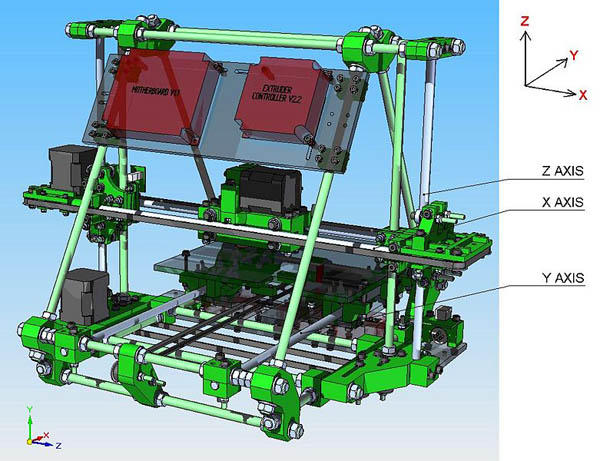
\includegraphics[scale=0.4]{Mendel_GA.jpg}
}

\frame{
  \frametitle{Leerdoel}
  \begin{itemize}
    \item<1-> Samenwerken (Open source)
    \item<2-> Software
    \item<3-> Hardware
    \item<4-> Documenteren (www.buildingmendel.nl)
  \end{itemize}
}

\frame{
  \frametitle{Voortgang}
  \begin{itemize}
    \item<1-> Frame gemaakt
    \item<2-> Afstellen
    \item<3-> Test prints
  \end{itemize}
  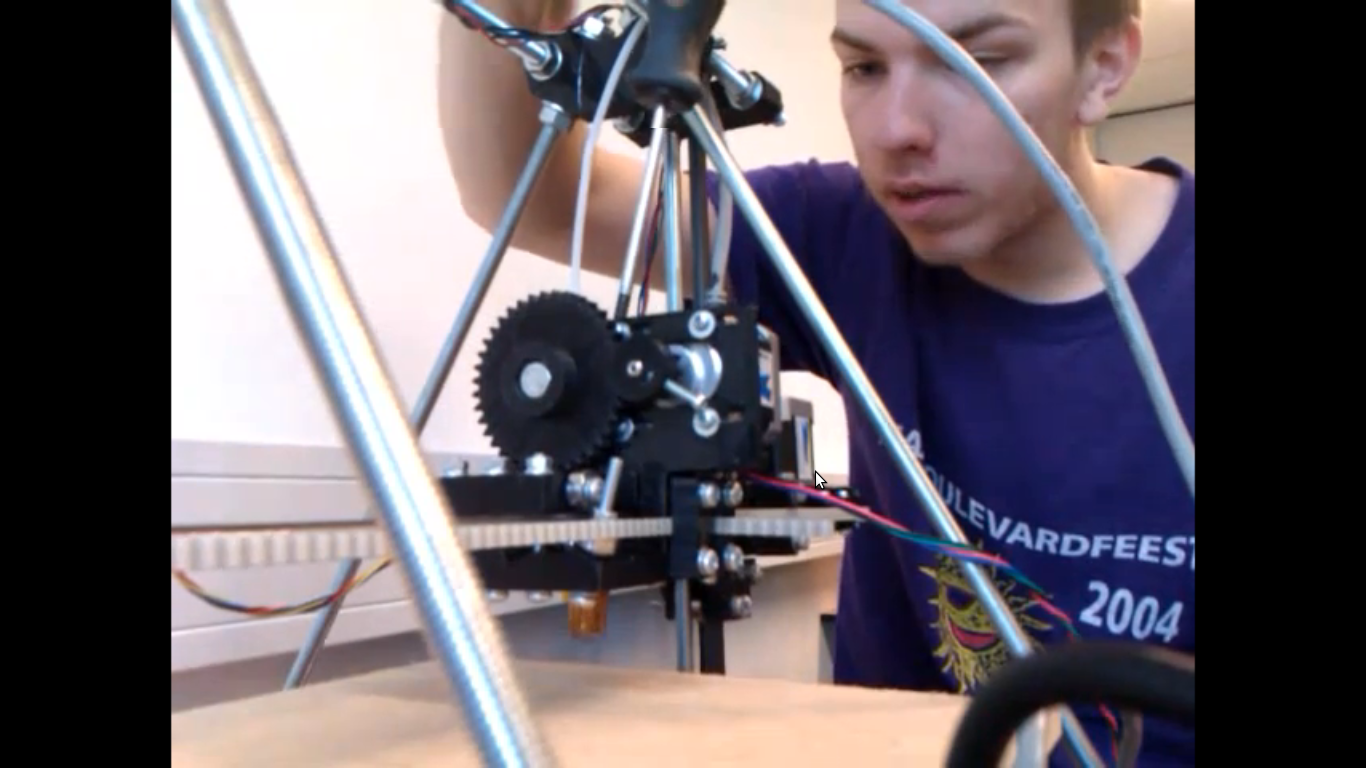
\includegraphics[scale=0.2]{Schermafdruk-1.png}
}

\frame{
  \includegraphics[scale=0.085]{IMG_0953_bwt.jpg}
}


\frame{
  \frametitle{Doorgave}
  \begin{itemize}
    \item<1-> Eerste jaars 
    \item<2-> Kennis overdracht
    \item<3-> Helpende hand
  \end{itemize}
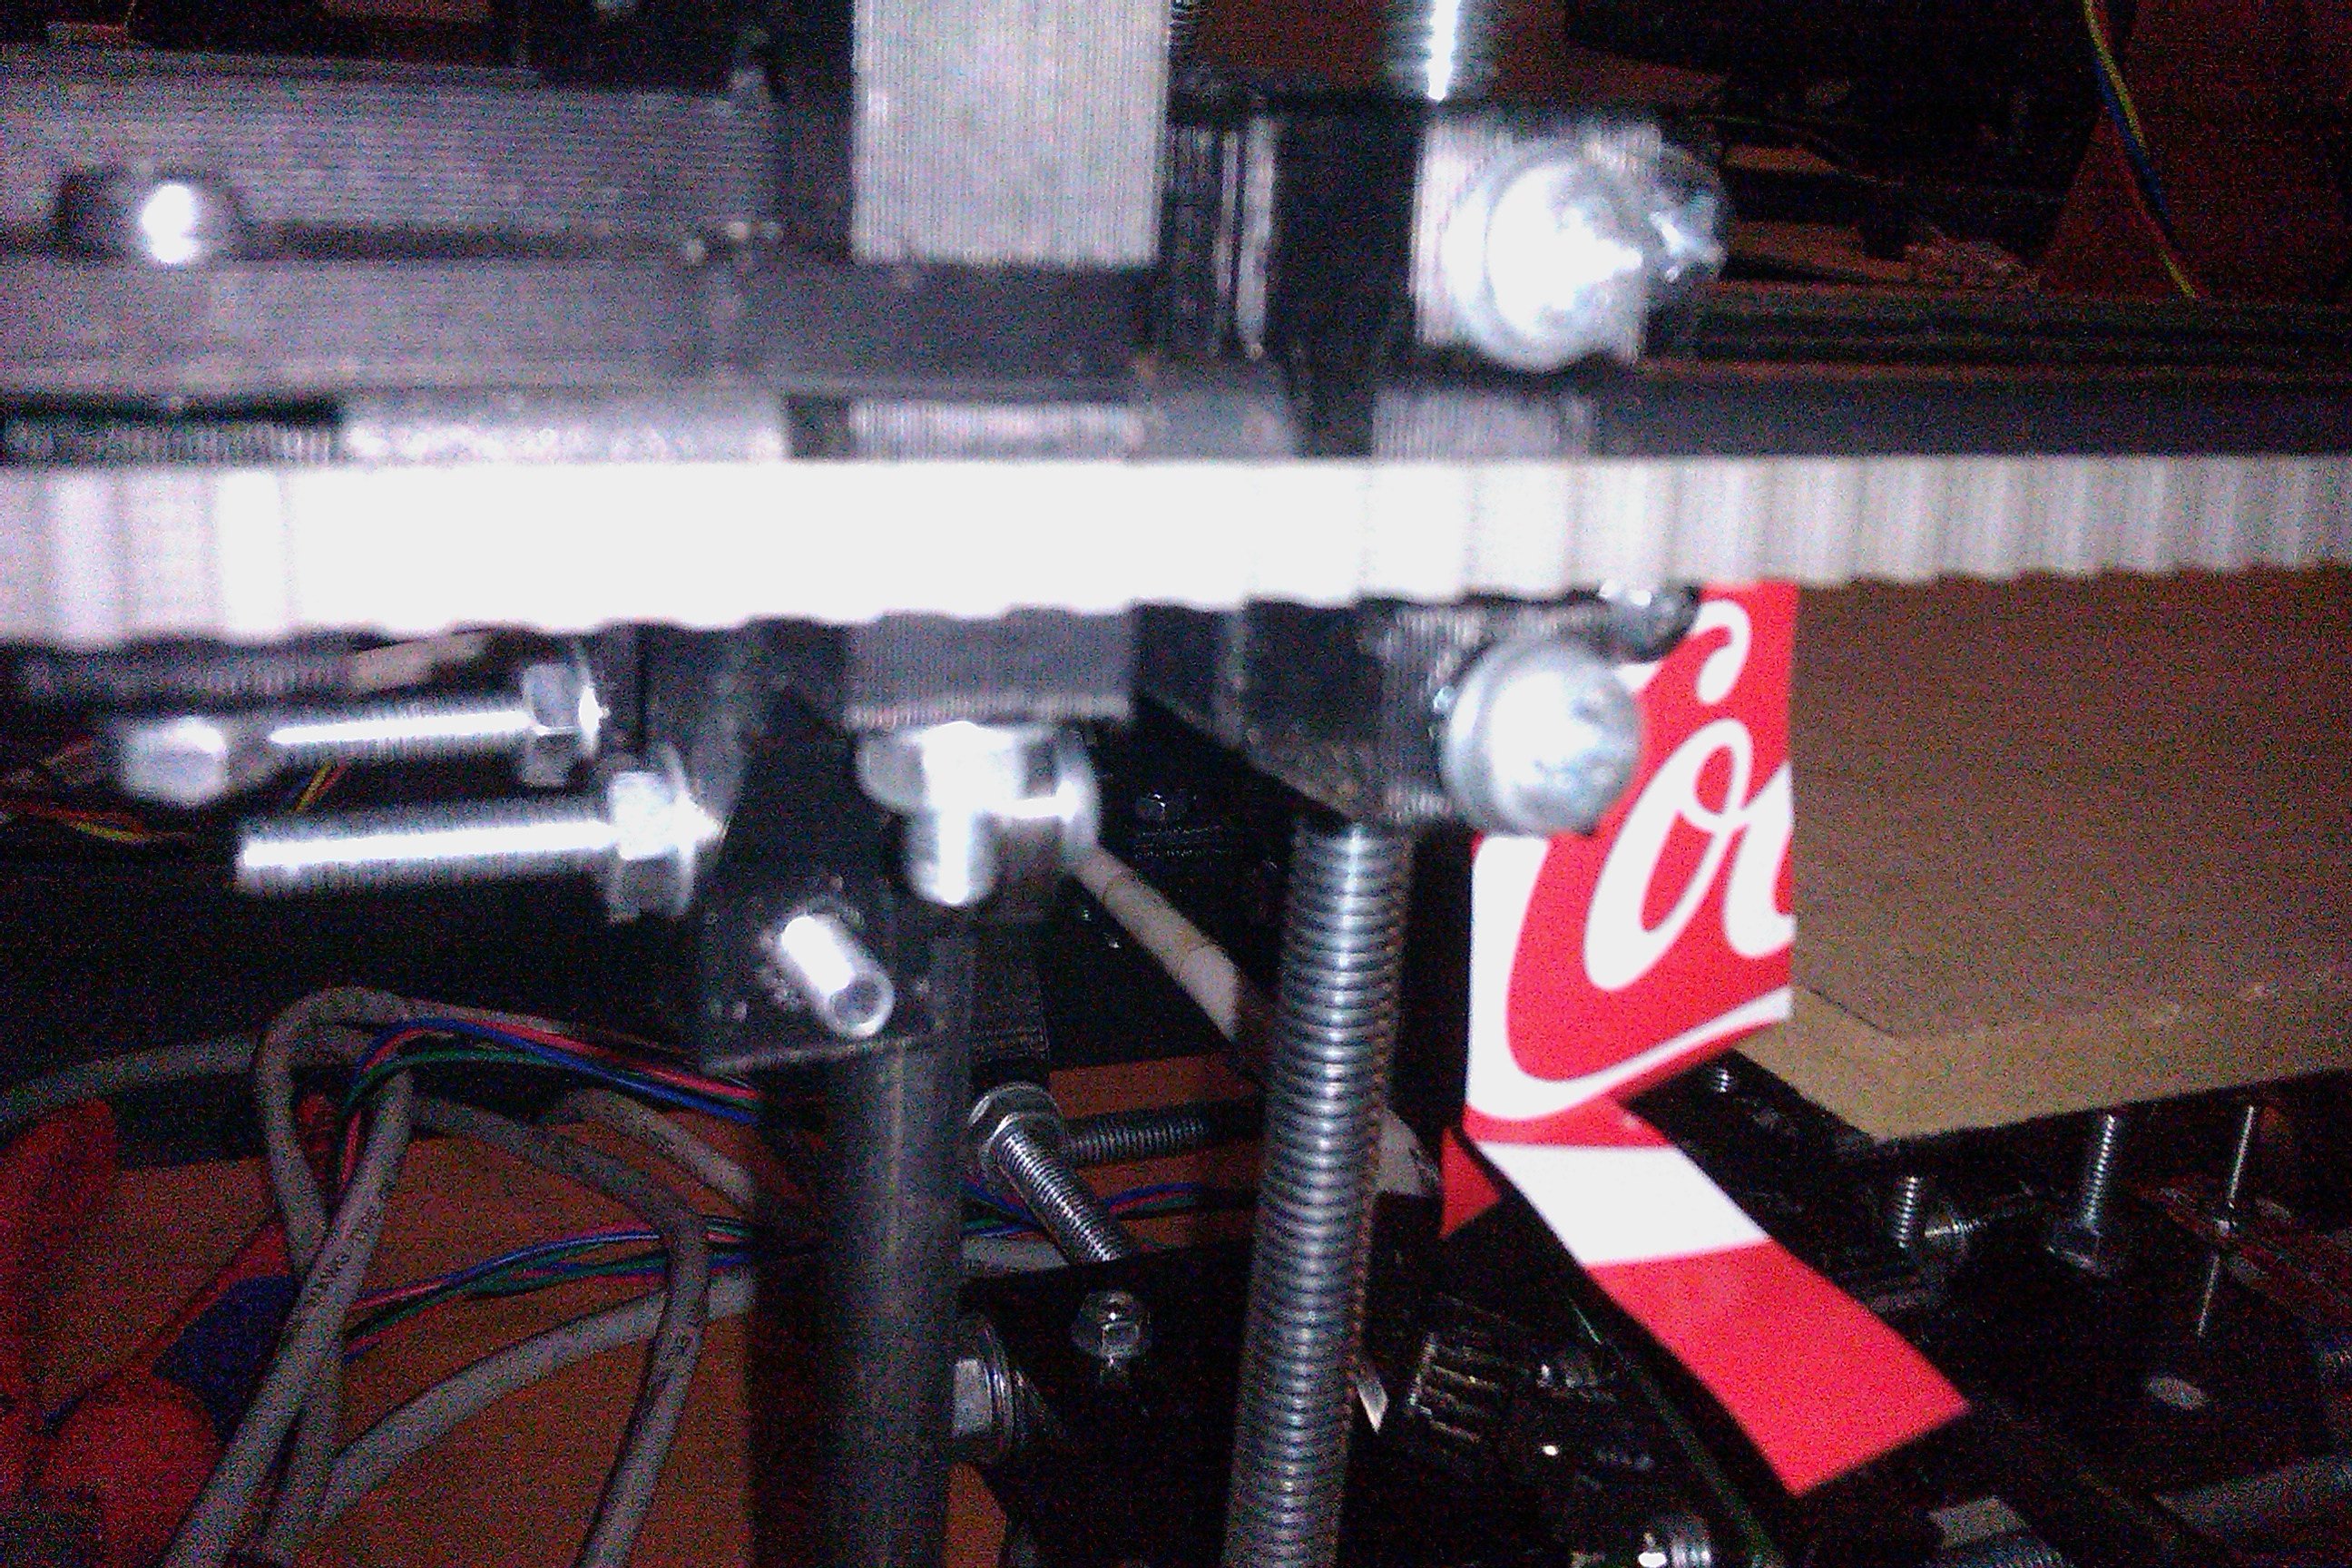
\includegraphics[scale=0.085]{imag0366.jpg}
}


\section{Afsluiting}
\frame{
  \frametitle{Afsluiting, zijn er nog vragen?} 
%  Zijn er nog vragen?
  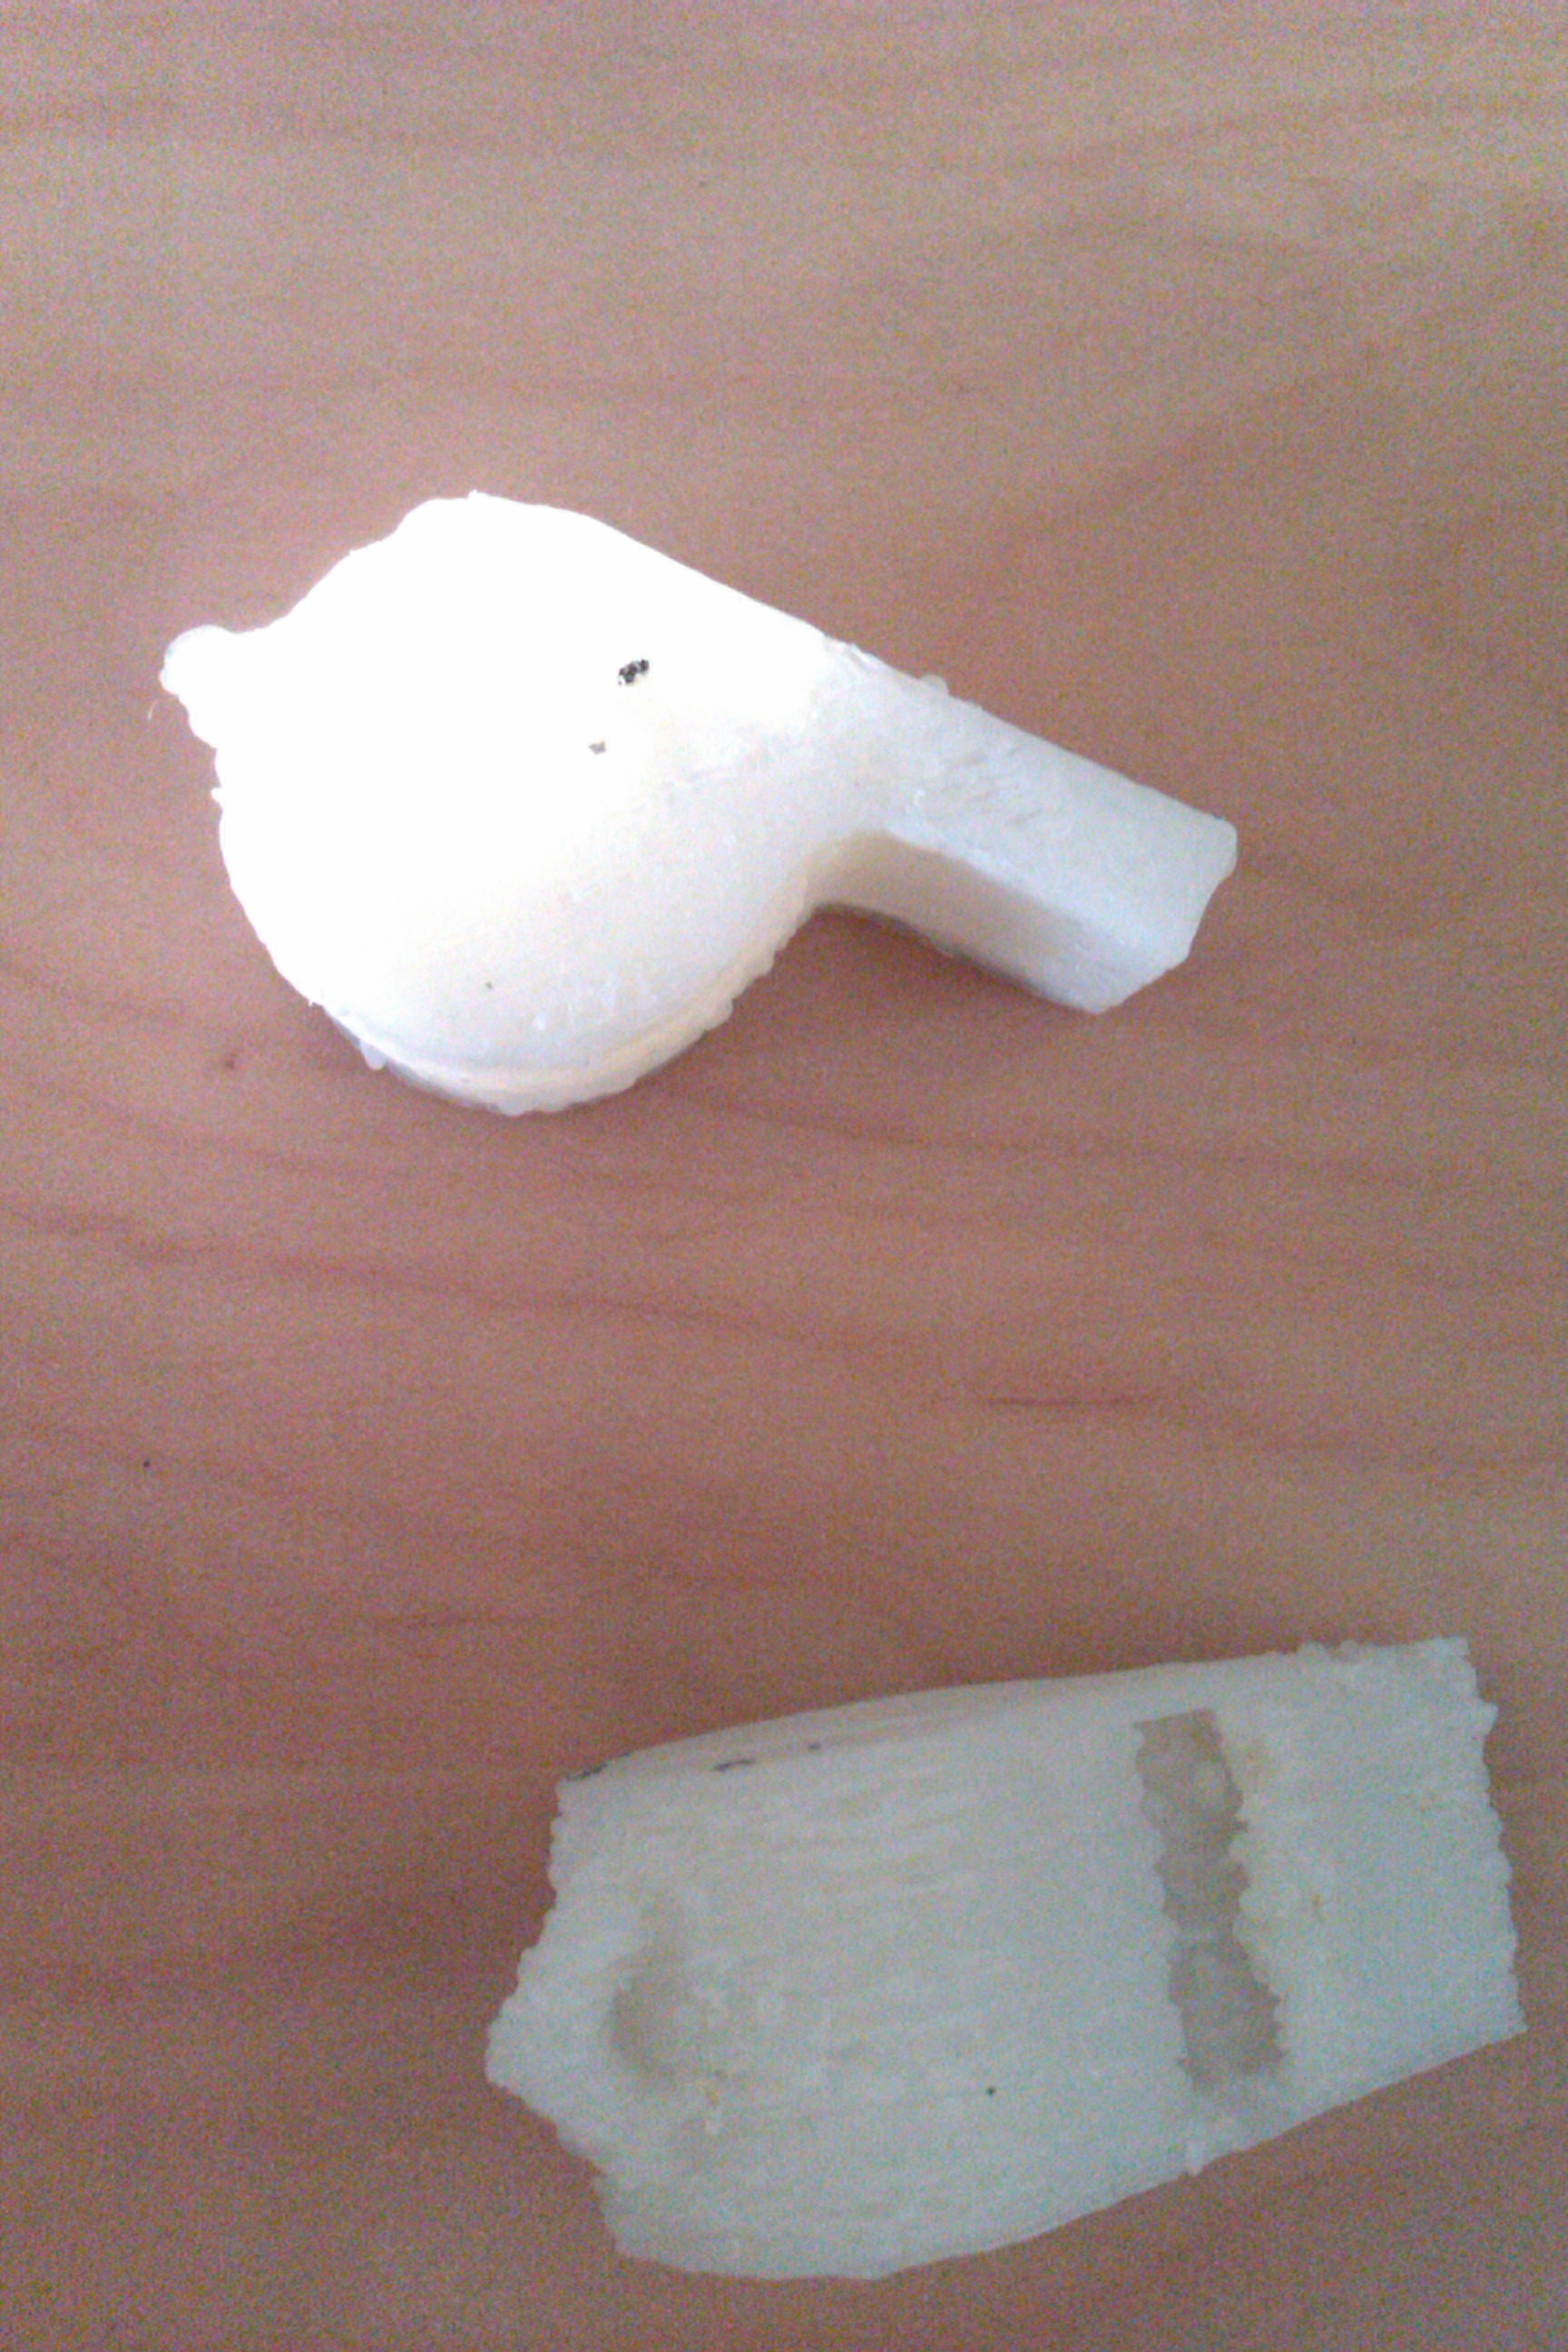
\includegraphics[scale=0.075]{IMAG0412.jpg}
}

\end{document}
